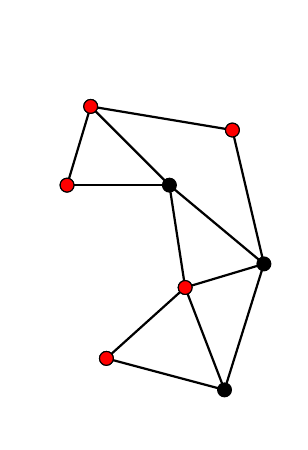
\begin{tikzpicture}
    \tikzstyle{vertex} = [draw=black,fill=black,circle,inner sep=0pt,minimum size=5pt];
    \tikzstyle{chosen} = [draw=black,fill=red,circle,inner sep=0pt,minimum size=5pt];
    \tikzstyle{edge} = [draw=black,thick];

    % This is an invisible rectangle which draw the picture to avoid nodes to move when appear/disappear.
    \path (0, 0) -- (3.2, 0) -- (3.2, 5) -- (0, 5);

    \coordinate (A) at (.5, 3);
    \coordinate (B) at (.8, 4);
    \coordinate (C) at (1, .8);
    \coordinate (D) at (1.8, 3);
    \coordinate (E) at (2, 1.7);
    \coordinate (F) at (2.5, 0.4);
    \coordinate (G) at (2.6, 3.7);
    \coordinate (H) at (3, 2);

    \node<2-5,7-> [style=vertex] at (A) {};
    \node<2-5,7-> [style=vertex] at (B) {};
    \node<2-5,7-> [style=vertex] at (C) {};
    \node<2-5,7-> [style=vertex] at (D) {};
    \node<2-5,7-> [style=vertex] at (E) {};
    \node<2-5,7-> [style=vertex] at (F) {};
    \node<2-5,7-> [style=vertex] at (G) {};
    \node<2-5,7-> [style=vertex] at (H) {};

    \draw<2-5,7-> [style=edge] (A) -- (B);
    \draw<2-5,7-> [style=edge] (A) -- (D);
    \draw<2-5,7-> [style=edge] (B) -- (D);
    \draw<2-5,7-> [style=edge] (B) -- (G);
    \draw<2-5,7-> [style=edge] (C) -- (E);
    \draw<2-5,7-> [style=edge] (C) -- (F);
    \draw<2-5,7-> [style=edge] (D) -- (E);
    \draw<2-5,7-> [style=edge] (D) -- (H);
    \draw<2-5,7-> [style=edge] (E) -- (F);
    \draw<2-5,7-> [style=edge] (E) -- (H);
    \draw<2-5,7-> [style=edge] (F) -- (H);
    \draw<2-5,7-> [style=edge] (G) -- (H);

    \node<4-7> [style=chosen] at (B) {};
    \node<4-7> [style=chosen] at (E) {};

    \node<8> [style=chosen] at (A) {};
    \node<8> [style=chosen] at (C) {};
    \node<8> [style=chosen] at (G) {};
\end{tikzpicture}